\documentclass[aps,pre,superscriptaddress,twocolumn,longbibliography]{revtex4-2}


% Common Package References
\usepackage{graphicx}
\usepackage{dcolumn}
\usepackage{bm}
\usepackage{epstopdf}
\usepackage{algorithm}
\usepackage{algpseudocode}
\usepackage[colorlinks]{hyperref}
\usepackage{amsmath,amsthm,amssymb}
\usepackage{float}
\usepackage{epsfig}
\usepackage{mathrsfs}
\usepackage{multirow}
\usepackage[all]{xy}
\usepackage{pbox}
\usepackage{verbatim}
\usepackage{braket}
\usepackage{mathtools}
\usepackage{tikz}
\usepackage{xcolor}
\usepackage{xfrac}
\usepackage{cleveref}

% Commenting commands

% Template below: replace 'initials' with your initials
%\newcommand{\initials}[1]{{\color{magenta}{\bf [INITIALS: #1]}}}


% Custom Commands
\newcommand{\singlefigure}{0.45\textwidth}


\begin{document}

% TITLE
\title{Drone Flight Controller, Project 9 - MLiS Part I}

% AUTHORS
\author{Jarrad Foley}
\email{ppxjf2@nottingham.ac.uk}
\affiliation{School of Physics and Astronomy, University of Nottingham, Nottingham, NG7 2RD, UK}
\author{Stephen McSweeney}
\email{ppxsm5@nottingham.ac.uk}
\affiliation{School of Physics and Astronomy, University of Nottingham, Nottingham, NG7 2RD, UK}

\date{\today}

\begin{abstract}
This paper outlines the process and intricacies that were explored with creating a drone that is controlled autonomously through reinforcement methods. The method implemented is a state-action value algorithm with a soft policy to ensure all states have a non-zero probability of being taken. This is kept to the bounds of a defined space and set of targets and a specified amount of timesteps. [RESULT] [CONCLUSION] % Loads the abstract.tex file
\end{abstract}

\maketitle

% SECTIONS
% Each section is written in a different file
\section{Introduction}
% Write your introduction here. One can cite\cite{ARXIVEXAMPLE} referenced in the \textit{references.bib} file.
Drones in the current age are becoming more and more popular making the public build their own versions of these drones from their homes. Usually drones are programmed with a flight controller to define how it moves for the task. While there are many ways to control a drone such as user controlled, this project focuses on implementing autonomous flight in which the drone will fly within a defined space to hit a number of targets. The drone that is to be controlled uses two motors which define the thrust independently allowing for navigation within the defined space. The task is to write a flight controller which uses reinforcement learning to have the drone traverse the space to hit as many targets as it can within a specified amount of time.


\section{Implementation}
For the implementation for this project we used a Soft policy Monti Carlo algorithm implementing a state-action value function ensuring that all actions can be taken with a non-zero probability. 

\subsection{States}
The states for this model uses the pitch of the drone, distance from the target both x and y, and velocity.
The State space used is 
$s={\left \{ Pitch, \Delta X, \Delta Y, V \right \}}$
Where each variable is discretized such that: pitch can take 30 values, X can take 40 values, Y can take 30 values, and Velocity can take 10 values. The total number of possible states is 360000.

\subsection{Actions}
There are 6 actions used within this program to define what movement the drone does.
\\
\begingroup\centering
$Ta =  \frac{1}{10}\max (-1,\min (10\Delta y,1))$

\endgroup

The first action is used to counteract the drones current pitch if it is facing the wrong direction from the target. 

\begingroup
$
T_1, T_2 = 
\left\{\begin{matrix}
    T_1 = \frac{1}{2}, T_2 = \frac{1}{2} & sgn(\Delta x) = sgn(\Theta ))

    \\ \\
    T_1 = \max (1,\min (\frac{sgn (\Delta x)}{2}+1),0)) & sgn(\Delta x) \neq sgn(\Theta ))
    & \\
    T_2 = \max (1,\min (-(\frac{sgn (\Delta x)}{2}+1)),0))
    \end{matrix}\right.$
\break
\endgroup

The second action adjusts the thrusts based on where the target is in the space and the angle of change that the drone will need to adjust to be directed at the target multiplied by 2. If the target is to the left of the drone it will have a lower left thrust than right thrust and vice versa. 

\begingroup\centering
$T_1 = \max (1,\min (\frac{2}{5}+Ta+2\Delta pitch,0))$
$T_2 = \max (1,\min (\frac{2}{5}+Ta-2\Delta pitch,0))$

\endgroup

The third action gets the thrust based on the velocity of the drone's pitch to adjust which thrust it needs more power to counteract the current rotation when it’s not rotating towards the target. This action is unstable compared to another action which does the same thing just at a slower rate.

\begingroup\centering

$T_1 = \frac{1}{2} - \frac{2}{5} sgn (pitchvelocity)$
$T_2 = \frac{1}{2} + \frac{2}{5} sgn (pitchvelocity)$

\endgroup

The fourth action changes the thrust depending on the current pitch velocity of the drone. If the pitch velocity is in the direction of the target then the thrusts will more equal to slow down how much it spins, however if the pitch velocity is going in the opposite direction of the target then it strongly sets the thrusts to alter the pitch velocity to be towards the target, spinning it into the correct direction.

\begingroup\centering
$
T_1, T_2 = 
$\left\{\begin{matrix}
    T_1 = \max (\frac{2}{5},\min (sign(\Delta x)),\frac{3}{5})) & sign(\Delta x) = sign(pitchvelocity))
    & \\
    T_2 = \max (\frac{2}{5},\min (sign(\Delta x)),\frac{3}{5}))
    \\ \\
    T_1 = \max (\frac{1}{5},\min (sign(\Delta x)),\frac{4}{5})) & sign(\Delta x) \neq sign(pitchvelocity))
    & \\
    T_2 = \max (\frac{1}{5},\min (sign(\Delta x)),\frac{4}{5}))
    \end{matrix}\right.$

\endgroup

The fifth action adjusts the thrusts based on where the target is in the space and the angle of change that the drone will need to adjust to be directed at the target. If the target is to the left of the drone it will have a lower left thrust than right thrust and vice versa. 

\begingroup\centering
$T_1 = \max (1,\min (\frac{1}{2}+Ta+\Delta pitch,0))$
$T_2 = \max (1,\min (\frac{1}{2}+Ta-\Delta pitch,0))$

\endgroup

The final action is used to adjust the drones y value. If the drones y value is lower than the target's y value then the drone will ascend and if the drones y value is above the target's y value then the drone will descend. 

\begingroup\centering
$T_1 =  \max (0,\min (sgn(\Delta y),1))$
$T_2 =  \max (0,\min (sgn(\Delta y),1))$

\endgroup

\subsection{Rewards}
We use the following reward function:

\begingroup\centering

$R=\frac{(-3a+0.1b-c+2d^3)}{100}$

\endgroup

Where:

\begingroup\centering
$a=\left \| Target Distance \right \|$

$b=abs(Drone Velocity)$

$c= \left \lfloor abs(DronePitch)  \right \rfloor $

$d=1+TargetsHit$

\endgroup

\section{Results}


Each assessment was done with the following target coordinates.

\begingroup
{\centering
    \begin{tabular}{|l|l|l|l|l|l|}
    \hline
    \textbf{Target} & \textbf{1} & \textbf{2} & \textbf{3} & \textbf{4} & \textbf{5}  \\ \hline
    \textbf{x}      & 0.35       & -0.35      & 0.5        & -0.35      & 0.35        \\ \hline
    \textbf{y}      & 0.3        & 0.4        & -0.4       & 0          & 0.4         \\ \hline
    \end{tabular}
    \begin{tabular}{|l|l|l|l|l|l|}
        \hline
        \textbf{Target} & \textbf{6} & \textbf{7} & \textbf{8} & \textbf{9} & \textbf{10} \\ \hline
        \textbf{x}      & -0.15      & -0.35      & 0.35       & -0.5       & 0.35        \\ \hline
        \textbf{y}      & -0.1       & -0.3       & -0.4       & 0.4        & 0           \\ \hline
        \end{tabular}
}
\endgroup


Each simulation was also run for 3000 simulation steps and 5000 epochs.

In this simulation, the heuristic algorithm hit 5 targets and achieved a value for the sum of rewards as 4894.42, against our chosen reward function.
The following graph shows an example of the Soft state Monti-Carlo state machine algorithm’s results, under the same conditions. \Cref{fig:fig1}.

We modelled the cumulative reward function for any given epoch using the least-squares optimized log function. \Cref{fig:fig1}.

The Logarithmic line for best fit is defined by the following equation:
\begingroup\centering
$1475.01044ln(0.00310817391CumReward) + 1642.65857$
\endgroup

The model has a residual standard deviation of 711.29847146. 
\begin{figure}
    \centering
    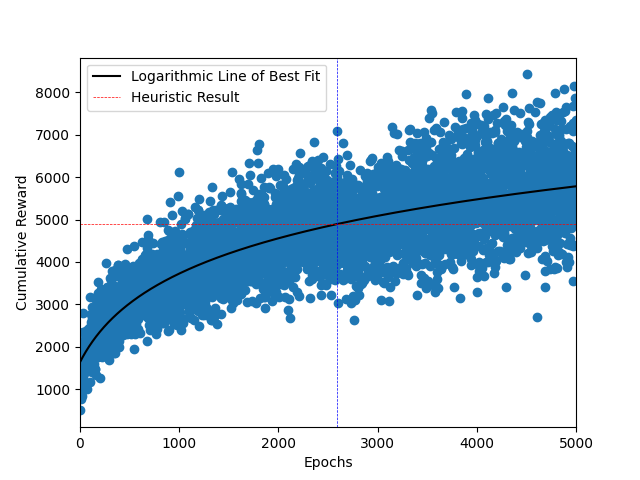
\includegraphics[width=\singlefigure]{figures/figure_2.png}
    \caption{\label{fig:fig1} Shows Logarithmic line of best fit of the data with result of the heuristic.}
\end{figure}

\begin{figure}
    \centering
    \includegraphics[width=\singlefigure]{figures/figure_3.png}
    \caption{\label{fig:fig2} Shows correlation between how many targets hit and cumulative reward for simulation.}
\end{figure}
\section{Evaluation}
Each assessment was done with the following target coordinates.

\begin{table}[]
    \begin{tabular}{|l|l|l|l|l|l|l|l|l|l|l|}
    \hline
    \textbf{Target} & \textbf{1} & \textbf{2} & \textbf{3} & \textbf{4} & \textbf{5} & \textbf{6} & \textbf{7} & \textbf{8} & \textbf{9} & \textbf{10} \\ \hline
    \textbf{x}      & 0.35       & -0.35      & 0.5        & -0.35      & 0.35       & -0.15      & -0.35      & 0.35       & -0.5       & 0.35        \\ \hline
    \textbf{y}      & 0.3        & 0.4        & -0.4       & 0          & 0.4        & -0.1       & -0.3       & -0.4       & 0.4        & 0           \\ \hline
    \end{tabular}
\end{table}

Each simulation was also run for 3000 simulation steps.

In this simulation, the heuristic algorithm hit 5 targets and achieved a value for the sum of rewards as 4894.42, against our chosen reward function.
The following graph shows an example of the Soft state Monti-Carlo state machine algorithm’s results, under the same conditions. This is not a deterministic algorithm and therefore there is some variance  between iterations.

We modelled the results for the sum of the reward function for any given epoch through minimising the error with a log function.


\section{Conclusions}

The ML alorithm sucessfully demonstrated logarithmic improvement over time.
The cumulative reward function was a successful indicator for the performance of the drone to the high correlation.
The model shows signs of outperforming the Heuristic model but more simulations are required to demonstrate this with statistical significance.
This was a limited of the time contraint of the project.

For future improvements to this work, more simulations are recommended and over more epochs to improve the model.
Through collecting data for different actions and state spaces, it may be possible to improve the performance of the model.


% BIBLIOGRAPHY
\appendix
\bibliography{references}

\end{document}